\usetikzlibrary{arrows.meta,calc,patterns}
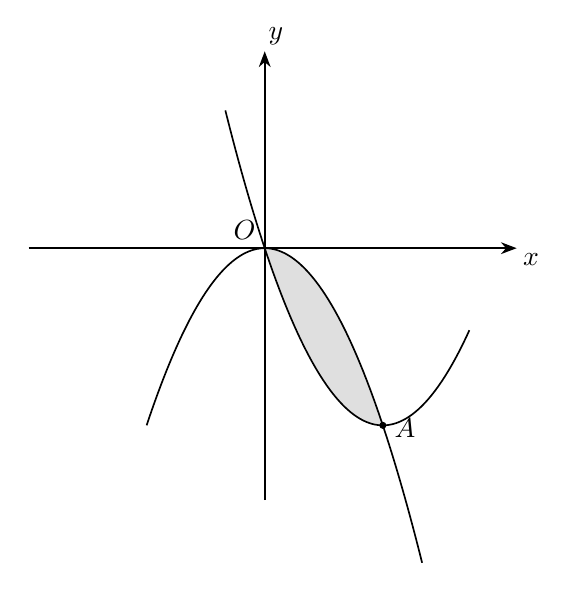
\begin{tikzpicture}[x=1cm,y=1cm,line width=.6pt,>=Stealth,font=\normalsize]
\draw[->] (-3.000000,0) -- (3.200000,0);
\node[anchor=west,inner sep=0pt,xshift=2.000000pt,yshift=-4.000000pt] at (3.200000,0) {$x$};
\draw[->] (0,-3.200000) -- (0,2.500000);
\node[anchor=south,inner sep=0pt,xshift=4.000000pt,yshift=2.000000pt] at (0,2.500000) {$y$};
\node[anchor=south east,inner sep=0pt,xshift=-3.000000pt,yshift=3.000000pt] at (0,0) {$O$};
\fill[gray!25] plot[domain=0:1.500000,samples=60] (\x,{-1*\x*\x}) -- plot[domain=1.500000:0,samples=60] (\x,{\x*\x-3.0*\x}) -- cycle;
% C1: y=-x^2
\draw[domain=-1.500000:2.000000,samples=101,smooth] plot (\x,{-1*\x*\x});
% C2: y=x^2-3x (a=1.5)
\draw[domain=-0.500000:2.600000,samples=101,smooth] plot (\x,{\x*\x-3.0*\x});
\fill (1.500000,-2.250000) circle (0.045000);
\node[anchor=west,inner sep=0pt,xshift=4.000000pt,yshift=-1.000000pt] at (1.500000,-2.250000) {$A$};
\end{tikzpicture}
